\section{各阶段炸弹破解与分析}
\begin{center}
    每阶段15分,密码10分,分析5分,总分不超过80分
\end{center}

\subsection{阶段1的破解与分析}

\textbf{密码如下:}I am not part of the problem. I am a Republican.

\textbf{破解过程:}

\begin{figure}[H]
\begin{minipage}[l]{0.5\linewidth}
\centering
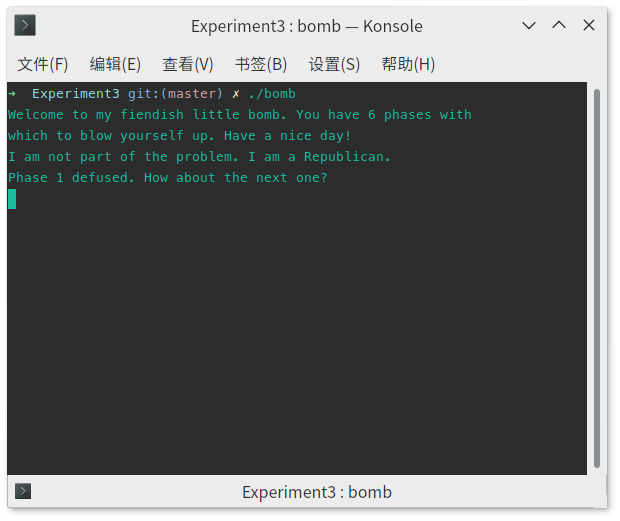
\includegraphics[width=\linewidth]{figures/Bomb-1}
\caption{阶段一}
\label{fig:bomb-1}
\end{minipage}
\begin{minipage}[r]{0.5\linewidth}
esi常作为参数使用,这里可以看到是比较字符串,推测0x402440是字符串地址,将其输出,发现确实是一串有意义的字符串,应该是答案一,测试成功。
\end{minipage}
\end{figure}


\subsection{阶段2的破解与分析}

\textbf{密码如下:}1 2 4 8 16 32

\textbf{破解过程:}

\begin{figure}[H]
    \begin{minipage}[l]{0.4\linewidth}
        \centering
        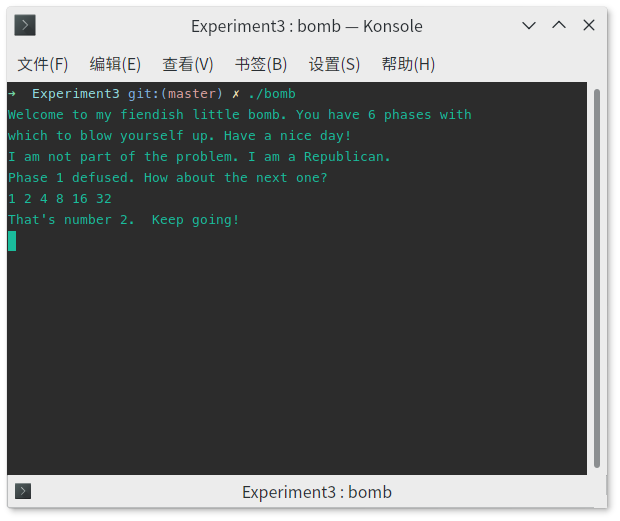
\includegraphics[width=\linewidth]{figures/Bomb-2}
        \caption{阶段二}
        \label{fig:bomb-2}
    \end{minipage}
    \begin{minipage}[r]{0.5\linewidth}
        看其汇编代码可知要我们输入的是6个数字,在读数完成之后可以发现,将rsp中的数据与1做了比较,不相等则爆炸,推测输入的地一个数字应该是1,之后则将eax赋值为ebx指向的值为1,在不读取完6个数字之前,每次eax做循环都会变成自己的2倍,然后与数组中的数据做比较,可得密码是1 2 4 8 16 32。
    \end{minipage}
\end{figure}

\subsection{阶段3的破解与分析}

\textbf{密码如下:}0 d 104

\textbf{破解过程:}

\begin{lstlisting}
0000000000400f0d <phase_3>:
400f0d:	48 83 ec 28          	sub    $0x28,%rsp
400f11:	64 48 8b 04 25 28 00 	mov    %fs:0x28,%rax
400f18:	00 00 
400f1a:	48 89 44 24 18       	mov    %rax,0x18(%rsp)
400f1f:	31 c0                	xor    %eax,%eax
# sscanf 将值存入到 rsp+14 rsp+16 rsp+10里面去了
# 只需要看这这三个值即可
# sprintf(in,"%d %c %d",%rdx,%rcx,%r8)
400f21:	4c 8d 44 24 14       	lea    0x14(%rsp),%r8
400f26:	48 8d 4c 24 0f       	lea    0x0f(%rsp),%rcx
400f2b:	48 8d 54 24 10       	lea    0x10(%rsp),%rdx
# 0x40249e 是"%d %c %d" 这就是要输入的三个值
400f30:	be 9e 24 40 00       	mov    $0x40249e,%esi
400f35:	e8 76 fc ff ff       	callq  400bb0 <__isoc99_sscanf@plt>
# 成功输入三个值,否则爆炸 %eax=3
400f3a:	83 f8 02             	cmp    $0x2,%eax
400f3d:	7f 05                	jg     400f44 <phase_3+0x37>
400f3f:	e8 82 05 00 00       	callq  4014c6 <explode_bomb>
400f44:	83 7c 24 10 07       	cmpl   $0x7,0x10(%rsp)
# rsp+10>7就爆炸
400f49:	0f 87 f2 00 00 00    	ja     401041 <phase_3+0x134>
# 把第一个数存到eax
400f4f:	8b 44 24 10          	mov    0x10(%rsp),%eax
# 0x4024b0的值是0x400f5a 
# 跳转到0x400f5a + rax * 8 (rax < 7)
# Switch 通过输入的第一个值进行跳转 这里输入0
400f53:	ff 24 c5 b0 24 40 00 	jmpq   *0x4024b0(,%rax,8)
# 0 :
# 0x68 : %d 第二个数字 0x68 = 104
400f5a:	b8 64 00 00 00       	mov    $0x64,%eax
400f5f:	83 7c 24 14 68       	cmpl   $0x68,0x14(%rsp)
400f64:	0f 84 e1 00 00 00    	je     40104b <phase_3+0x13e>
400f6a:	e8 57 05 00 00       	callq  4014c6 <explode_bomb>
400f6f:	b8 64 00 00 00       	mov    $0x64,%eax
400f74:	e9 d2 00 00 00       	jmpq   40104b <phase_3+0x13e>
# -*- 其它选项 -*-
# 将中间字母和al做比较
# 输入 0 : %eax = %al = 0x64 = d 中间的字母是 d
# 答案 0 d 104
40104b:	3a 44 24 0f          	cmp    0xf(%rsp),%al
40104f:	74 05                	je     401056 <phase_3+0x149>
\end{lstlisting}

\subsection{阶段4的破解与分析}

\paragraph{密码如下:}132 4

\paragraph{破解过程:}

\begin{lstlisting}
0000000000401070 <func4>:
# func4(a,b)
401070:	85 ff                	test   %edi,%edi
# if b <= 0 return 0;
401072:	7e 2b                	jle    40109f <func4+0x2f>
401074:	89 f0                	mov    %esi,%eax
401076:	83 ff 01             	cmp    $0x1,%edi
# if b ==1 return a;
401079:	74 2e                	je     4010a9 <func4+0x39>
40107b:	41 54                	push   %r12
40107d:	55                   	push   %rbp
40107e:	53                   	push   %rbx
40107f:	89 f5                	mov    %esi,%ebp
401081:	89 fb                	mov    %edi,%ebx
401083:	8d 7f ff             	lea    -0x1(%rdi),%edi
# c = func4(a,b-1)
401086:	e8 e5 ff ff ff       	callq  401070 <func4>
40108b:	44 8d 64 05 00       	lea    0x0(%rbp,%rax,1),%r12d
401090:	8d 7b fe             	lea    -0x2(%rbx),%edi
401093:	89 ee                	mov    %ebp,%esi
# c += func4(a,b-2)
401095:	e8 d6 ff ff ff       	callq  401070 <func4>
# return a+c
40109a:	44 01 e0             	add    %r12d,%eax
40109d:	eb 06                	jmp    4010a5 <func4+0x35>
40109f:	b8 00 00 00 00       	mov    $0x0,%eax
4010a4:	c3                   	retq   
4010a5:	5b                   	pop    %rbx
4010a6:	5d                   	pop    %rbp
4010a7:	41 5c                	pop    %r12
4010a9:	f3 c3                	repz retq 

00000000004010ab <phase_4>:
4010ab:	48 83 ec 18          	sub    $0x18,%rsp
4010af:	64 48 8b 04 25 28 00 	mov    %fs:0x28,%rax
4010b6:	00 00 
4010b8:	48 89 44 24 08       	mov    %rax,0x8(%rsp)
4010bd:	31 c0                	xor    %eax,%eax
4010bf:	48 89 e1             	mov    %rsp,%rcx
4010c2:	48 8d 54 24 04       	lea    0x4(%rsp),%rdx
# 0x40260f:"%d %d"
# sscanf(in,"%d %d",%rdx,%rcx)
# sscanf(in,"%d %d",%rsp+4,%rsp)
4010c7:	be 0f 26 40 00       	mov    $0x40260f,%esi
4010cc:	e8 df fa ff ff       	callq  400bb0 <__isoc99_sscanf@plt>
4010d1:	83 f8 02             	cmp    $0x2,%eax
4010d4:	75 0b                	jne    4010e1 <phase_4+0x36>
4010d6:	8b 04 24             	mov    (%rsp),%eax
4010d9:	83 e8 02             	sub    $0x2,%eax
4010dc:	83 f8 02             	cmp    $0x2,%eax
# (%rsp + 4) <= 4 否则爆炸
4010df:	76 05                	jbe    4010e6 <phase_4+0x3b>
4010e1:	e8 e0 03 00 00       	callq  4014c6 <explode_bomb>
4010e6:	8b 34 24             	mov    (%rsp),%esi
4010e9:	bf 07 00 00 00       	mov    $0x7,%edi
# %eax = func4(%esi,%edi)
# %eax = func4(%rsp+4,7)
4010ee:	e8 7d ff ff ff       	callq  401070 <func4>
4010f3:	3b 44 24 04          	cmp    0x4(%rsp),%eax
4010f7:	74 05                	je     4010fe <phase_4+0x53>
4010f9:	e8 c8 03 00 00       	callq  4014c6 <explode_bomb>
4010fe:	48 8b 44 24 08       	mov    0x8(%rsp),%rax
401103:	64 48 33 04 25 28 00 	xor    %fs:0x28,%rax
40110a:	00 00 
40110c:	74 05                	je     401113 <phase_4+0x68>
40110e:	e8 ed f9 ff ff       	callq  400b00 <__stack_chk_fail@plt>
401113:	48 83 c4 18          	add    $0x18,%rsp
401117:	c3                   	retq   
\end{lstlisting}

\begin{lstlisting}[language = c]
//func_4可等价为如下函数
int func_4(int a, int b) {
  if (b <= 0)
    return 0;
  if (b == 1)
    return a;
  return a + func(a, b - 1) + func(a, b - 2);
}
\end{lstlisting}


\subsection{阶段5的破解与分析}

\paragraph{密码如下:}gamfeg

\paragraph{破解过程:}

\begin{lstlisting}
0000000000401118 <phase_5>:
401118:	53                   	push   %rbx
401119:	48 83 ec 10          	sub    $0x10,%rsp
40111d:	48 89 fb             	mov    %rdi,%rbx
401120:	64 48 8b 04 25 28 00 	mov    %fs:0x28,%rax
401127:	00 00 
401129:	48 89 44 24 08       	mov    %rax,0x8(%rsp)
40112e:	31 c0                	xor    %eax,%eax
# 判断字符长度 不等于6则爆炸
401130:	e8 74 02 00 00       	callq  4013a9 <string_length>
401135:	83 f8 06             	cmp    $0x6,%eax
401138:	74 05                	je     40113f <phase_5+0x27>
40113a:	e8 87 03 00 00       	callq  4014c6 <explode_bomb>
# %eax = 0
40113f:	b8 00 00 00 00       	mov    $0x0,%eax
# %rbx -> "输入的字符串"
# %rdx -> "输入的字符串"
401144:	0f b6 14 03          	movzbl (%rbx,%rax,1),%edx
# %rdx 取低4位
401148:	83 e2 0f             	and    $0xf,%edx
# 0x4024f0:"maduiersnfotvbylSo you think you can stop the bomb with ctrl-c, do you?"
# 查表取得值,表项如下
# maduiersnfotvbyl
# 0123456789abcdef
40114b:	0f b6 92 f0 24 40 00 	movzbl 0x4024f0(%rdx),%edx
401152:	88 14 04             	mov    %dl,(%rsp,%rax,1)
401155:	48 83 c0 01          	add    $0x1,%rax
401159:	48 83 f8 06          	cmp    $0x6,%rax
40115d:	75 e5                	jne    401144 <phase_5+0x2c>
40115f:	c6 44 24 06 00       	movb   $0x0,0x6(%rsp)
# 0x4024a7:"sabres"
# 推出表项  71d657
# IN:       gamfeg
# 只需输入的字母的ASCII码的低8位和表项值相同即可
401164:	be a7 24 40 00       	mov    $0x4024a7,%esi
401169:	48 89 e7             	mov    %rsp,%rdi
40116c:	e8 56 02 00 00       	callq  4013c7 <strings_not_equal>
401171:	85 c0                	test   %eax,%eax
401173:	74 05                	je     40117a <phase_5+0x62>
401175:	e8 4c 03 00 00       	callq  4014c6 <explode_bomb>
40117a:	48 8b 44 24 08       	mov    0x8(%rsp),%rax
40117f:	64 48 33 04 25 28 00 	xor    %fs:0x28,%rax
401186:	00 00 
401188:	74 05                	je     40118f <phase_5+0x77>
40118a:	e8 71 f9 ff ff       	callq  400b00 <__stack_chk_fail@plt>
40118f:	48 83 c4 10          	add    $0x10,%rsp
401193:	5b                   	pop    %rbx
401194:	c3                   	retq   
\end{lstlisting}

\subsection{阶段6的破解与分析}

\paragraph{密码如下:}3 6 4 2 1 5

\paragraph{破解过程:}
\begin{lstlisting}
0000000000401195 <phase_6>:
401195:	41 55                	push   %r13
401197:	41 54                	push   %r12
401199:	55                   	push   %rbp
40119a:	53                   	push   %rbx
40119b:	48 83 ec 68          	sub    $0x68,%rsp
40119f:	64 48 8b 04 25 28 00 	mov    %fs:0x28,%rax
4011a6:	00 00 
4011a8:	48 89 44 24 58       	mov    %rax,0x58(%rsp)
4011ad:	31 c0                	xor    %eax,%eax
4011af:	48 89 e6             	mov    %rsp,%rsi
4011b2:	e8 31 03 00 00       	callq  4014e8 <read_six_numbers>
4011b7:	49 89 e4             	mov    %rsp,%r12
4011ba:	41 bd 00 00 00 00    	mov    $0x0,%r13d
# while(true){
4011c0:	4c 89 e5             	mov    %r12,%rbp
4011c3:	41 8b 04 24          	mov    (%r12),%eax
4011c7:	83 e8 01             	sub    $0x1,%eax
# %rbp = %r12 -> "1 2 3 4 5 6"
# %r13d = 0
# %eax = *(%r12)-1
# 每个数 都小于等于 6
4011ca:	83 f8 05             	cmp    $0x5,%eax
4011cd:	76 05                	jbe    4011d4 <phase_6+0x3f>
4011cf:	e8 f2 02 00 00       	callq  4014c6 <explode_bomb>
# %r13d += 1
# if(%r13d == 0x6) goto LABEL2
#   break;
4011d4:	41 83 c5 01          	add    $0x1,%r13d
4011d8:	41 83 fd 06          	cmp    $0x6,%r13d
4011dc:	74 3d                	je     40121b <phase_6+0x86>
# %ebx = %r13d
4011de:	44 89 eb             	mov    %r13d,%ebx
# %rax = %ebx * 2
# do{
4011e1:	48 63 c3             	movslq %ebx,%rax
# %eax = &(%rsp + %rax * 4)
4011e4:	8b 04 84             	mov    (%rsp,%rax,4),%eax
4011e7:	39 45 00             	cmp    %eax,0x0(%rbp)
# if(%eax == %rbp) bomb
4011ea:	75 05                	jne    4011f1 <phase_6+0x5c>
4011ec:	e8 d5 02 00 00       	callq  4014c6 <explode_bomb>
4011f1:	83 c3 01             	add    $0x1,%ebx
4011f4:	83 fb 05             	cmp    $0x5,%ebx
4011f7:	7e e8                	jle    4011e1 <phase_6+0x4c>
# %ebx += 1
# }while(ebx <= 5); 每个数都不相等
4011f9:	49 83 c4 04          	add    $0x4,%r12
4011fd:	eb c1                	jmp    4011c0 <phase_6+0x2b>
# } 
# 输入的数字是1-6的全排列
# { 将链表中的数据按照你输入的值取出到 %rsp+24之上
# node = node -> next
# {
4011ff:	48 8b 52 08          	mov    0x8(%rdx),%rdx
# %eax ++
401203:	83 c0 01             	add    $0x1,%eax
# %eax == %ecx ?
401206:	39 c8                	cmp    %ecx,%eax
401208:	75 f5                	jne    4011ff <phase_6+0x6a>
# }访问链表的各个节点,找到你输入的数字所对应序号的节点
# *(%rsp+0x20+2*%rsi) = %rdx
# 将链表的指针存入栈中
40120a:	48 89 54 74 20       	mov    %rdx,0x20(%rsp,%rsi,2)
40120f:	48 83 c6 04          	add    $0x4,%rsi
401213:	48 83 fe 18          	cmp    $0x18,%rsi
401217:	75 07                	jne    401220 <phase_6+0x8b>
401219:	eb 19                	jmp    401234 <phase_6+0x9f>
#LABEL2:
40121b:	be 00 00 00 00       	mov    $0x0,%esi
# %ecx中存入的是你所输入的值
401220:	8b 0c 34             	mov    (%rsp,%rsi,1),%ecx
401223:	b8 01 00 00 00       	mov    $0x1,%eax
# 0x6032f0是个链表的头
#   地址   | 内容  | 序号 |   next  
# 0x6032f0 : 0x100   0x01   next-> 0x603300
# 0x603300 : 0x12e   0x02   next-> 0x603310
# 0x603310 : 0x234   0x03   next-> 0x603320
# 0x603320 : 0x139   0x04   next-> 0x603330
# 0x603330 : 0x0b9   0x05   next-> 0x603340
# 0x603340 : 0x142   0x06   next-> NULL
# 3 6 4 2 1 5
401228:	ba f0 32 60 00       	mov    $0x6032f0,%edx
40122d:	83 f9 01             	cmp    $0x1,%ecx
401230:	7f cd                	jg     4011ff <phase_6+0x6a>
401232:	eb d6                	jmp    40120a <phase_6+0x75>
#  }
401234:	48 8b 5c 24 20       	mov    0x20(%rsp),%rbx
401239:	48 8d 44 24 20       	lea    0x20(%rsp),%rax
40123e:	48 8d 74 24 48       	lea    0x48(%rsp),%rsi
401243:	48 89 d9             	mov    %rbx,%rcx
# %rbx = node[0]
# %rax = node
# %rsi = node[6]
# %rcx = %rbx
# do{
# %rdx = node[x] -> next
401246:	48 8b 50 08          	mov    0x8(%rax),%rdx
40124a:	48 89 51 08          	mov    %rdx,0x8(%rcx)
40124e:	48 83 c0 08          	add    $0x8,%rax
401252:	48 89 d1             	mov    %rdx,%rcx
401255:	48 39 f0             	cmp    %rsi,%rax
401258:	75 ec                	jne    401246 <phase_6+0xb1>
# }while(%rax != %rsi);
# 取得一个数组value[6]中存的是取出的各节点存储的值,按照所输入的数据取出
40125a:	48 c7 42 08 00 00 00 	movq   $0x0,0x8(%rdx)
401261:	00 
401262:	bd 05 00 00 00       	mov    $0x5,%ebp
401267:	48 8b 43 08          	mov    0x8(%rbx),%rax
40126b:	8b 00                	mov    (%rax),%eax
40126d:	39 03                	cmp    %eax,(%rbx)
# 把每个数字和它的下一个数字做比较 当前的数字要大于下一个数字,否则爆炸
# 按值取出序号可得:3 6 4 2 1 5
40126f:	7d 05                	jge    401276 <phase_6+0xe1>
401271:	e8 50 02 00 00       	callq  4014c6 <explode_bomb>
401276:	48 8b 5b 08          	mov    0x8(%rbx),%rbx
40127a:	83 ed 01             	sub    $0x1,%ebp
40127d:	75 e8                	jne    401267 <phase_6+0xd2>
40127f:	48 8b 44 24 58       	mov    0x58(%rsp),%rax
401284:	64 48 33 04 25 28 00 	xor    %fs:0x28,%rax
40128b:	00 00 
40128d:	74 05                	je     401294 <phase_6+0xff>
40128f:	e8 6c f8 ff ff       	callq  400b00 <__stack_chk_fail@plt>
401294:	48 83 c4 68          	add    $0x68,%rsp
401298:	5b                   	pop    %rbx
401299:	5d                   	pop    %rbp
40129a:	41 5c                	pop    %r12
40129c:	41 5d                	pop    %r13
40129e:	c3                   	retq   
\end{lstlisting}

\subsection{阶段7的破解与分析(隐藏部分)}

\paragraph{密码如下:}

\paragraph{破解过程:}
